% arara: pdflatex: { shell: yes }
\documentclass[a4paper,10pt]{article}
\usepackage[margin=1in]{geometry}
\usepackage{titlesec}
\usepackage{hyperref}
\usepackage{enumitem}
\usepackage{graphicx}
\usepackage{xcolor}

% Set link color to classic blue and underline
\hypersetup{
    colorlinks=true,
    linkcolor=black,
    urlcolor=blue,
    citecolor=black,
    filecolor=black
}

% Formatting section titles
\titleformat{\section}{\large\bfseries}{}{0em}{}
\titleformat{\subsection}{\bfseries}{}{0em}{}

\begin{document}


\begin{center}
    {\LARGE \textbf{Erick Gonzalez Parada}} \\
    \vspace{0.3cm}
    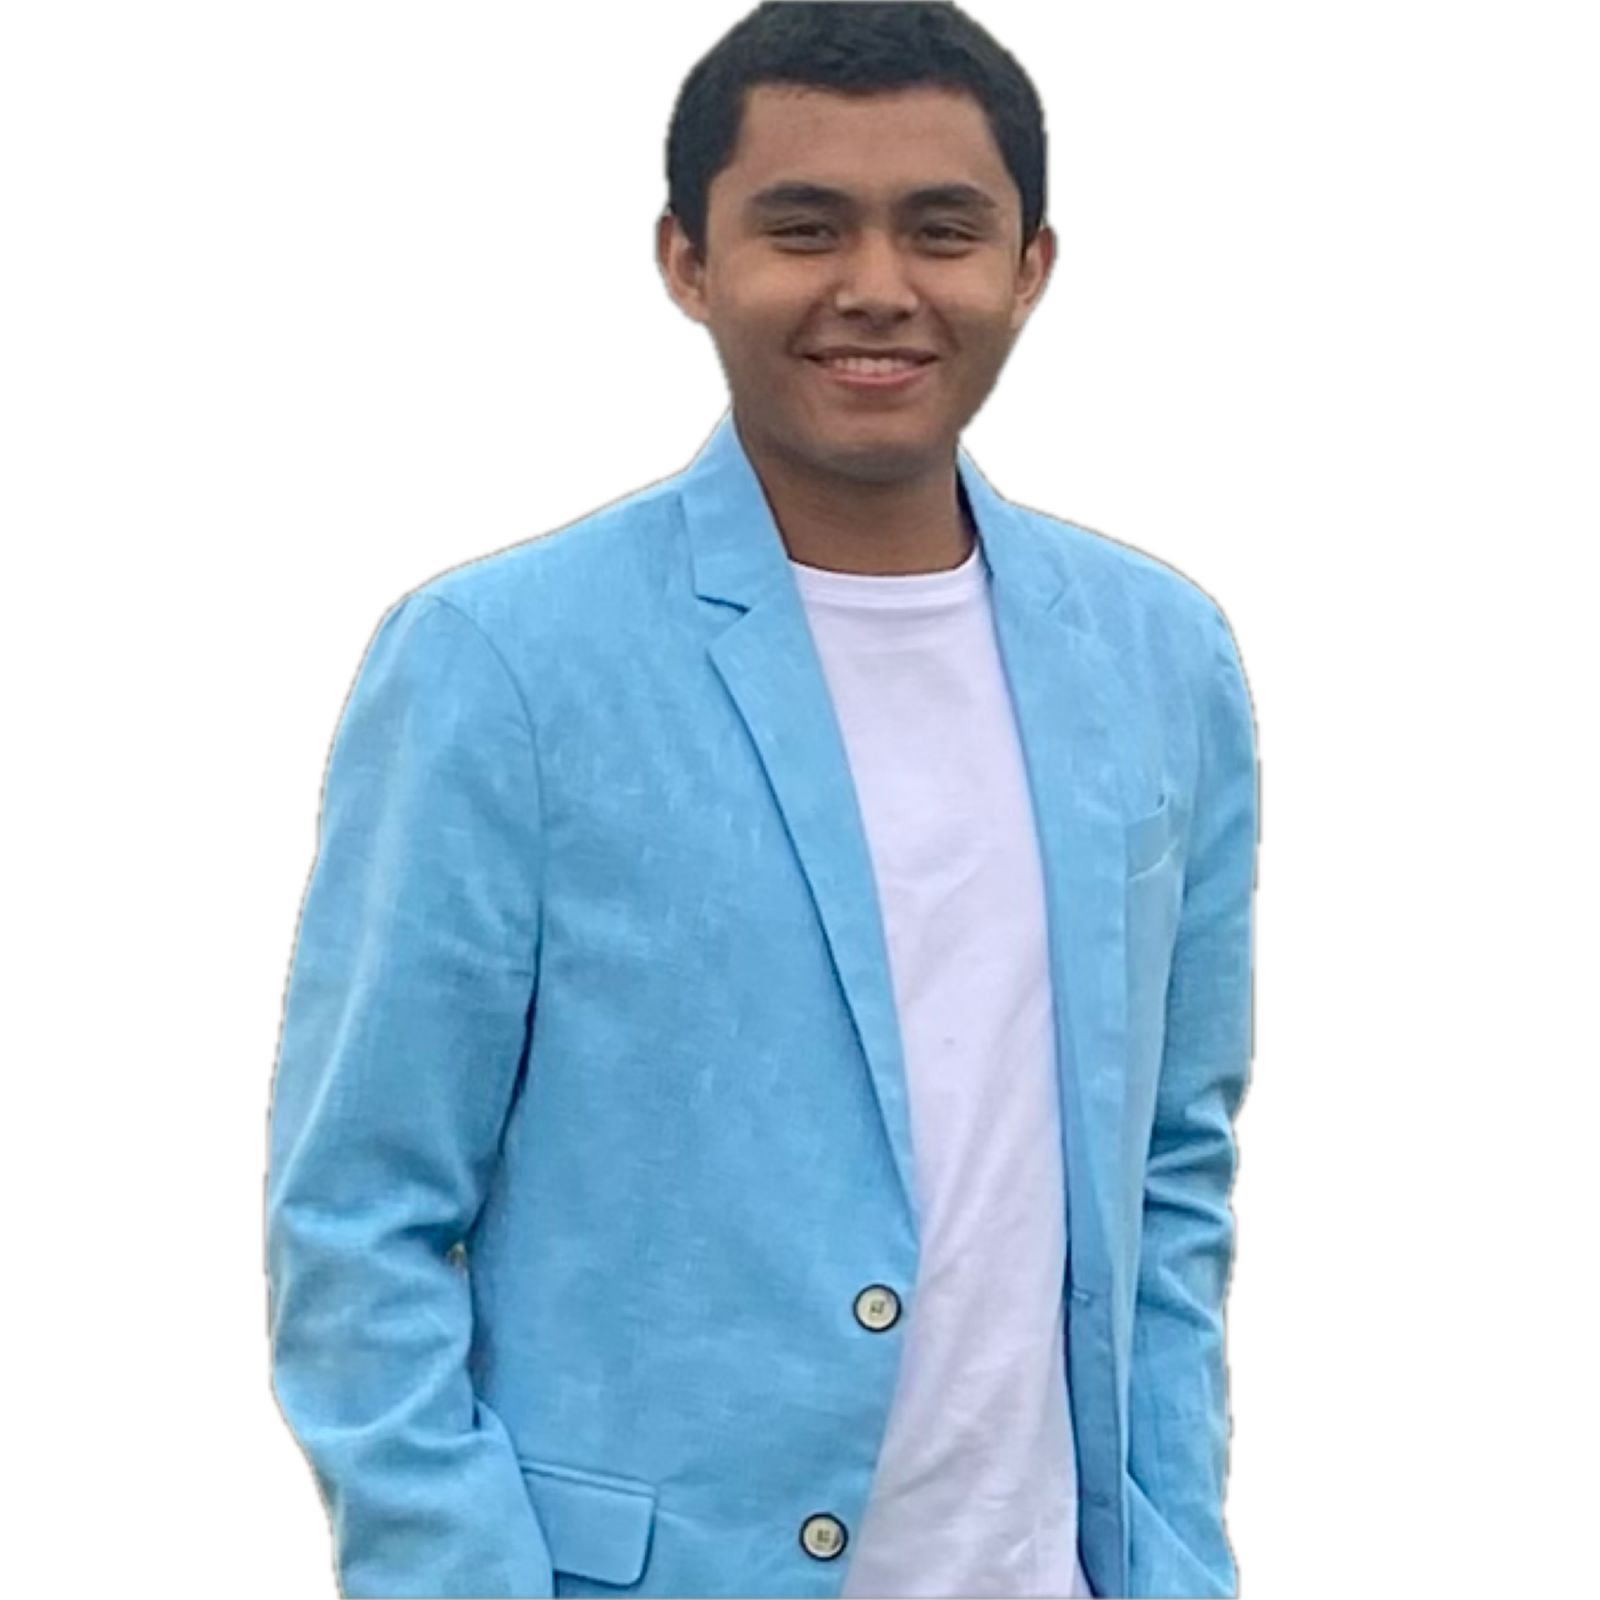
\includegraphics[width=3cm]{profpic.jpeg} \\
    \vspace{0.3cm}
    Puebla, Mexico $\cdot$ \underline{\href{https://linkedin.com/in/erick-gonzalez-810883335}{linkedin.com/in/erick-gonzalez-810883335}} \\
    +52 2228498841 $\cdot$ \underline{\href{mailto:erick.parada101@gmail.com}{erick.parada101@gmail.com}}
\end{center}



\section*{Summary}
I'm a software developer with expertise in full-stack development (both web and desktop). I love making my software available on all operating system platforms and have an interest in cybersecurity. Passionate about Linux, competitive programming, and chess. Currently a student at UDLAP (Universidad de las Américas Puebla), set to graduate in 2026.

\section*{Projects}
\subsection*{Unwanted Search Engine (GUI)}
\begin{itemize}
    \item Developed \textit{Unwanted Search Engine}, a lightweight, privacy-focused desktop search application using Rustlang and Raylib.
    \item Designed an interactive GUI with a responsive search bar, real-time feedback, and results display.
    \item Built a custom backend API integration for dynamic search result fetching and display.
\end{itemize}

\subsection*{Courses Academy Video Platform (Web Full-Stack)}
\begin{itemize}
    \item Developed a platform (JavaScript) where users can view courses created by administrators. Admins can add videos and manage other admins.
    \item Implemented CI/CD practices using Git and GitHub to improve efficiency, reducing bugs and delivery times.
    \item Designed user authentication flows on the frontend using JWT (e.g., login, signup, token storage, and renewal).
\end{itemize}


\section*{Education}
\textbf{Universidad de las Américas Puebla (UDLAP)}\\
\textit{Computer Systems Engineering}\\
Recognition: Interim Board of Computer Systems Engineering; Event Coordinator\\
Cholula, Mexico | Graduate May 2026

\section*{Additional Skills}
\begin{itemize}
    \item \textbf{Languages:} Spanish (native), English (100\%), German (70\%)
    \item \textbf{Programming:} C/C++, Rust, Java, JavaScript/TypeScript, Nextjs, Sveltejs, SQL (Postgresql), OQL, XML, Bash \& Batch
    \item \textbf{Technologies:} Linux, GitHub, CI/CD, Web Development
    \item \textbf{Profiles:} \underline{\href{https://github.com/HugeErick}{GitHub}}, \underline{\href{https://portafolio-delta-wheat.vercel.app/}{Web Portfolio}}
\end{itemize}

\end{document}

